\documentclass[12pt]{article}

% --------------------
% Basic Packages
% --------------------
\usepackage[a4paper,margin=1in]{geometry}
\usepackage{setspace}
\usepackage{graphicx}
\usepackage{amsmath}
\usepackage{amssymb}
\usepackage{longtable}
   \usepackage{array}
   \usepackage{xcolor}
   \usepackage{colortbl}
   \usepackage{tikz}
\usetikzlibrary{shapes, arrows.meta, positioning}
\usepackage{float}

\onehalfspacing

% --------------------
% Title and Author
% --------------------
\title{Intrusion Detection Mechanisms for Wireless
and IoT Networks}
\author{N KARTHEEK}
\date{}

\begin{document}
	\maketitle
	
	\section{Introduction}
	The modern digital environment has been evolving fast with the spread of wireless communication technologies and Internet of Things (IoT) ecosystem that allow connecting heterogeneous devices, sensors, actuators, and intelligent systems via pervasive communication. Embedded computation in combination with wireless networking has enabled massive applications in smart homes, medical monitoring devices, industrial automation systems, environmental sensors systems, smart transportation systems, and smart cities. All these interrelated environments are constantly producing, passing and processing enormous volumes of information, enabling real time decision making and autonomous processes. Nevertheless, over the past years, the scale of wireless IoT solutions applications has greatly exposed critical infrastructures to cybersecurity threats and as such, security assurance has become a default research and engineering issue [1], [2].



Wireless and IoT environments will be open and use a decentralized communication environment as opposed to a traditional wired enterprise network. Wireless networks are by their very nature broadcast, which means that opposed parties can capture, modify, or introduce malicious packets without necessarily obtaining straddling access to network infrastructure. More so, the IoT networks are often comprised of resource-constrained devices that have limited processing power, memory, and battery life. These limitations limit the use of computational heavy cryptographic tools and continuous monitoring systems at the device level. The lack of communication barriers, topological dynamism, heterogeneity of protocols, and limited resources present a complicated security environment that requires enormous protection measures [3], [4].



Traditional security preventive tools such as encryption, authentication, routine routing protocols and access control policies are the much needed initial layer of protection. Nonetheless, these mechanisms are not adequate and cannot ensure full protection. The vulnerabilities can be due to software defects, configuration mistakes, insider threats, compromised credentials, firmware attacks or zero-day attacks which can go around preventive mechanisms. Since every wireless IoT system is growing in size and complexity, the likelihood of successful intrusion is high. In turn, the intrusion detection mechanisms have become an important complementary element of the security that attempts to reveal malicious actions that are not noticed by the preventative measures [5], [6].



Intrusion Detection Systems-IDS It is a system that is created to check the trends of network traffic, protocol actions, and device-level activity so as to identify malicious access attempts, unusual system activity, or the violation of policy. The IDS solutions used in the context of wireless and IoT networks need to be efficient in the framework of distributed and heterogeneous network structures and are required to have a high detection rate and high false alarm rates. Their architecture needs a sizeable concern over the latency children, communication overhead, energy efficiency, along with the scalability. The detection of the known attack signatures and hitherto unexplored anomalies is of great significance in the IoT ecosystems where attack signatures are rapidly evolving and high volumes of devices are simultaneously connected at all times [7], [8].



Threat in wireless IoT network is of very broad nature, with numerous attack vectors that can potentially affect various protocol layers. At both the physical level and medium access level, the attackers can introduce jamming or collision-based denial of service attacks which, in turn, disrupt communication channels. Attack to routing and sinkhole attacks are attacks that can be used to weaken data forwarding paths through network layer. The threats at the application-layer are malware injection, data modification, and unauthorized command execution. In industrial and healthcare facilities, effective intrusions can result in not only breaching of data, but also operational interruptions and even a safety risk. These risks in multiple dimensions highlight the need of intelligent and adaptive schemes of detection with the capacity to exist in network layers [9], [10].



In the last years, the focus of research on advancing intrusion detection structures in wireless IoT networks has shifted towards the incorporation of machine learning and deep learning methods. The data-driven models are able to examine intricate traffic data and be trained to comprehend behavioral representation that facilitates the identification of small variations to the normal activity. The use of supervised classification models, unsupervised anomaly detection methods and the use of hybrid learning systems have been seen to show an encouraging difference in the detection accuracy. However, datasets imbalance issues, model generalization, interpretability, computational cost, and adverse effects to adversarial manipulation are important research challenges. Recent methods have thus necessitated optimized architectures and lightweight utilization of feature extraction techniques [11], [12] in the deployment of learning-based IDS in resource-restricted IoT settings.



Besides centralized architectures of detectors, distributed and collaborative intrusion detection architectures have been suggested to limit issues of scalability and latent. The paradigms provided by edge computing enable to process traffic data further to its source and consume less bandwidth and less time. Model training at scale and global threat intelligence aggregation are offered on cloud-assisted frameworks. The issue of finding an efficient balance between the responsiveness of the decentralization concept and the ability to differentiate centralization and analysis is a crucial design issue in current wireless IoT security systems [13], [14].



Due to the tendency to involve IoT systems into the work of cyber-physical infrastructures and industrial control systems, the significance of efficient intrusion detection is only going to rise. The security measures should maintain confidentiality, integrity of data, as well as maintain system availability and operational integrity. The dynamic integration of wireless communication technology, embedded intelligence, and the use of artificial intelligence-based analytics introduces the vulnerabilities and novel defensive possibilities. Thus, scalable, flexible, and resource efficient intrusion detection mechanisms are of primary focus when developing secure wireless and IoT ecosystems [15], [16].



Under this chapter, intrusion detection mechanisms specifically designed to be applied to wireless and IoT networks are considered in terms of their concept, methodology, the main features of their development, their applications, the open problems, and the development trends. In this systematic investigation, an in-depth comprehension of detection tactics that can be deployed in distributed and resource-constrained wireless settings is formulated.
	

	\section{Background and Conceptual Foundations}
	Designing of intrusion detection systems on a wireless and IoT network has a history that is rooted on the foundations of network security, the distributed system, and the wireless communication theory. Before researching advanced detection structures and clever techniques it is crucial to interpret these conceptual premises. Wireless IoT eco-systems are very different topologically compared to traditional wired infrastructures, dynamics of communication and operational constraint. These differences exist in design, implementation and testing of intrusion detection structures [1], [3].



\subsection{Evolution of Wireless and IoT Security Paradigms}



The early phases of network security were mainly the perimeter security models in which the firewalls and centralized monitoring systems were deployed to provide security to enterprise systems. The latter however with the introduction of the wireless networking technologies brought about open channels of communication that could not be confined in merely by physical isolation. The resources to mobile and ad hoc wireless worlds instead of the rudimentary wired networks required new security premises and spy techniques.



The security paradigm shifted further nearer to the distributed and heterogeneous ecosystems as the IoT architectures were presented. The IoT networks refer to a network of sensory devices, gate ways, cloud-based solutions as well as application platforms that rely on different protocol layers. This type of increase in architecture presented fresh risks of weaknesses in the machine authentication, the integrity of the firmware, manipulation of the routing and the confidentiality of the information. The intrusion detection systems, in their turn, have evolved into distributed context-sensitive systems of inspecting traffic that can be successful in a wide range of environments [4], [6].



The increasingly active impetus of IoT in the industrial control systems and cyber-physical infrastructures added to the need to have the real-time capabilities of detection even further. The breach of complexity of such systems through digital information and physical processes may influence the intrusion. Therefore, existing intra-detection technologies are expounded on to trace deviations in system fronting the network boundary in association with cognizance of deviation in system level action [7], [9].



\subsection{Rudimentary terms of the Intrusion Detection Systems}



One security feature is the Intrusion Detection System which monitors the activity that occurs on a network, system or even an application with an aim of identifying some form of suspicious activity which may be an indicator of bad intent. The IID solutions can be installed on other structures besides the host based structures, network based structuration and hybrid structure. Local monitoring of the devices and centralized or edge-aided analytics is a common feature of the wireless IoT systems that have a tradeoff between the accuracy in detection and computational efficiency [5], [10].



Intrusion detection techniques can be of three general types namely; signature-based detection, anomaly-based detection and specification-based detection. Signature based systems are based on prior knowledge of the attack and is effective in familiar attacks of intrusion. The anomaly based approaches establish a behavioral threshold as well as detecting abnormal behavior and enabling it to detect novel or rootkit attacks. Specification based detection sets out the rule of acceptable conduct and the violation of rule is identified as potential intrusions. Multi-method models involve the use of multiple methods with the intention of improving reliability and reducing false alarms.



The wireless IoT mandates IDS frameworks to take into consideration dynamic network topologies, low resource ability of devices and existence of heterogeneous communication protocols. The normal operation of the detection process is data collection, feature extraction, behaviour modelling, decision-making logic and alert generation. The effectiveness of all the steps depends on how well the characterization of traffic has been done and the dynamism applied in the algorithm of detecting the change in the network factors [8], [11].
	
	% ---- Figure (Generic Conceptual Diagram)
	\begin{figure}[h]
		\centering
		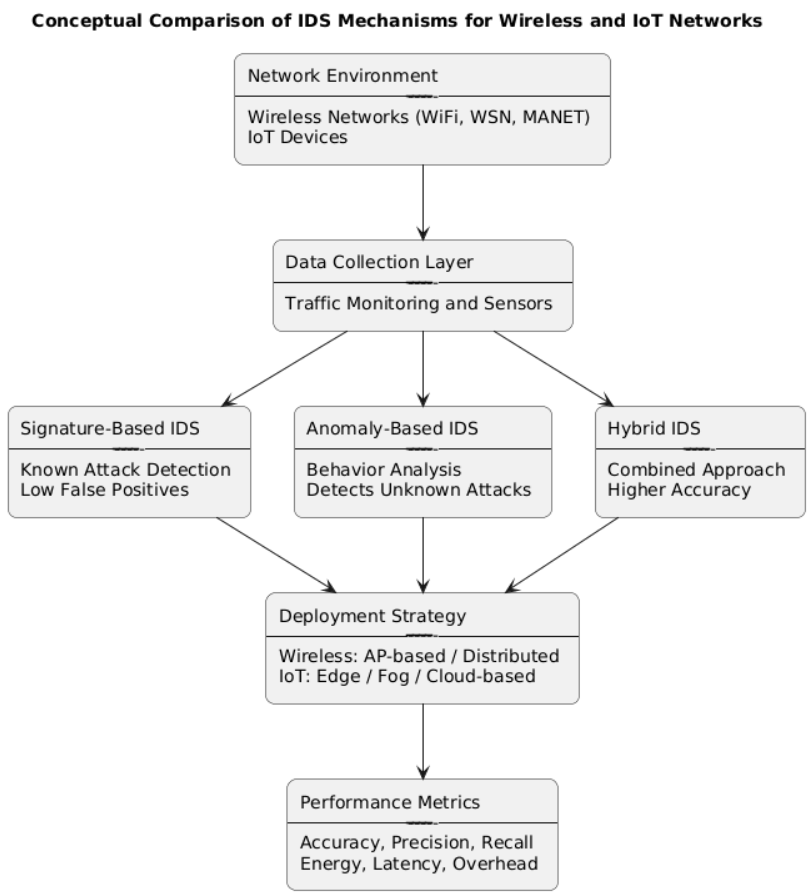
\includegraphics[width=0.75\textwidth]{IDS.png}
		\caption{Conceptual Comparison of IDS Mechanisms for Wireless and IoT Networks}
		\label{fig:conceptual_overview}
	\end{figure}
	
	% ---- Table (Generic Terminology / Concepts Table)
	\begin{table}[h]
\centering
\caption{Representative Concepts in Wireless IoT Intrusion Detection}
\label{tab:concepts}
\begin{tabular}{|p{3cm}|p{8cm}|}
\hline
\textbf{Concept} & \textbf{Description} \\
\hline
Core Entity & Primary sensing or computing device participating in the wireless IoT network, responsible for data generation, sensing, and communication. \\
\hline
Communication Unit & Wireless protocol or transmission mechanism enabling data exchange among IoT devices, gateways, and cloud infrastructure. \\
\hline
Detection Engine & Analytical module that processes traffic features or behavioral metrics to identify suspicious or malicious activities. \\
\hline
Control Logic & Decision-making component responsible for evaluating detection results and initiating alerts or mitigation responses. \\
\hline
Operational Constraint & Resource or environmental limitation such as energy capacity, bandwidth availability, latency sensitivity, or computational capability. \\
\hline
\end{tabular}
\end{table}

\subsection{Architectural Components in Wireless IoT Environments}	
Wireless IoT intrusion detection framework systems consist of various interconnected layers that with each other, can facilitate surveillance activities, format and response activities. Compared to the scheme of the traditional enterprise network where the impetus is concentrated in the centralized places of checking, the space of the IoT is decentralized in nature and multifaceted. The layout of the intrusion detection systems will however have the capacity to cope with decentralized locating of the devices, non-uniform communication protocols along with shifting traffic plans. The layer application of the detection tasks is commonly devised providing the device, edge, and cloud level by practicing an architectural perspective.















IoT devices produce sensing data, and provide the involvement of wireless communication on the equipment layer. Such devices and smart meters and industrial control are required in the cyber-physical systems, which can include environmental sensors, wearable use and industrial control. Intrusion detection schemes at device level are often implemented in order to execute lightweight surveillance applications, e.g. counting packets, anomaly detection based on a threshold value or by a rule, due to power and computation constraints. Localization of detection is better able to boost the responsiveness; however, it has to be well planned so that it does not add up too much of processing load to the apparatus and hence negative impact on response [11], [12].















The identity of the IoT devices and the centralized cloud services is an intermediate layer referred to as an edge or a gateway layer. The other devices also collect and can calculate fairly in comparison to the individual sensors as well as accumulate the traffic in the edge nodes. This layer is capable of sustaining more sophisticated ways of characterizing features and modeling behaviors in parallel at minimal latency. The bandwidth was also saved heavily by the implementation of edge assisted intrusion detection designs to filter the data so that it could only be sent to the centralized systems. They also scale these designs to a large extent but also permit close to real-time detection in applications where latency plays a role like industrial automation and also load monitoring in healthcare processes [13], [14].















The huge processing and training of the models is typically done at the cloud or centralized analysis model. The high-performance computing is used to power the intrusion detection systems of the clouds to crunch the aggregated traffic patterns, functioning of the global threat intelligence databases, and the continuous updates of the detection models. The situation between a centralized analytics and distributed-monitoring coincide to create the top-down system of finding that is more effective in respect to computational effectiveness and detection accuracy. Its dependence on infrastructural centralization, however, might be associated with some privacy-related issues and possible failures point some of which can be managed by generating well-structured patterns of coordination between the aspects of architecture [15], [16].















These layers interact based on the communication protocols, data aggregation and response coordination mechanisms policies. Elements of control logic refer to how alerts that are agreed at various levels are confirmed and increased. Layers likewise are aligned to contribute to the effectiveness of such architectures and dynamism is also provided in such architecture to respond to dynamically changing the network topologies. The architectural flexibility as well as modularity are some of the most important design aspects of sustainable intrusion detection models with respect to the dynamism of the wireless IoT ecosystems.


\subsection{Threat Model and Attack Surface in Wireless IoT Networks}
The adversarial capabilities with the multi-layered attack surfaces are the features of the threat landscape of wireless IoT networks. The overall model of threats should be capable of actualizing both the foreign attackers who would take advantage of the wireless communication mediums, and the internal attackers, who would target the legitimate devices. The disadvantage of wireless transmission is that it is a menace to passive eavesdropping and active interference to network progression because of the characteristics of broadcast of this mode of transmissions. The hacks can enter the system with a weak authentication system, system firmwares or unsuitable communication standards, without the necessary authorization [7], [9].















The attackers can establish jamming attacks, interference with the transmission of the signals or collision-based denial-of-service attacks in the physical and medium access control layers, an act which is simply a wastage of the communication resources. These jamming affect the availability of the networks negatively and, in the case of using live times, may be, to a considerable extent, affected. Since the general IoTs implementations consist of most of them being in low-powered wide-area networks or short range wireless connections, any form of interference will negatively affect the quality of services delivered.















It can be attacked by network layers like sinkholes attacks, selective forwarding attacks and spoofing attacks that interfere with the pathways of delivering data. The disseminated topologies of IoTs of the compromised nodes can be updated with the routing information to direct traffic towards the malicious intermediaries to be circumvented. Besides being able to intercept the data it is also possible to corrupt or drop the packets, which will most likely result to data integrity and reliability issues [10], [14].















There are also threats of the application layer extended to the extent of attack. Firsthand influence on the operating of the gadgets can be related to intrusion of malware, unauthorized alteration of firmed code (being able to convert the firmware of a PC or the work of other machinery), utilisation of data and command execution etc. Such tradeoffs can lead to erroneous actuation commands, or necessary interrupts to the industrial and healthcare IoT setting. These threats are even more fearful since the cyber and the physical are merged and the breaches of the cybersecurity are turned into the safety threats.















The other type of significance of the IoT threat model is the large scale coordinated attacks like the creation of botnets. The compromised and attenuated IoT devices can be ordered to be used without being present physically to be used to engage in the distributed denial-of-service attacks of the external infrastructure. The embedded security controls that are inherent to majority of the low cost IoT-driven devices are comparatively low in number implying they are open to the mass exploitation. The intrusion detection mechanisms must then be able to detect some deviant traffic patterns which will be indicative of orchestrated malevolent behaviors by a group of individuals.















All that and dynamical and heterogeneous model of the IoT ecosystems complicate the threat modelling. These devices are constantly being added or removed to networks, new version changing firmware is being released to other deployments and traffic is constantly changing. The forces make constant behaviour levels levels of anomaly detection systems hard to attain. This implies that the adaptive models should be obliged to enable intrusion detection in wireless IoT networks in order to enable the prospect of the multi-layers observation and reacting to dynamically-evolving attack plans [12], [16].

	\section{Core Concepts and Approaches}
	The wireless and IoT networking intrusion detection landscape has taken a dramatic turn under the influence of specific challenges that these fields have. The study has proven the existence of three key conceptual foundations that characterize modern solutions to the securing of such distributed, resource-limited networks.



\subsection{Machine Learning and Deep Learning Architectures}
    The academic area has demonstrated how willing people are to use innovative and advanced neural networks to solve IoT and wireless security issues. Deep learning has become a prominent trend and the Long Short Term Memory (LSTM) framework has been identified as an effective way to identify temporal attributes of network traffic. Combining CNN and LSTM models utilises both spatial and sequential characteristics, while the use of more developed attention mechanisms allows for greater emphasis on the associated features of the traffic involved. Areas of research interest being pursued by researchers include custom architectures such as the L2D2 LSTM model, designed for identifying multi-class intrusion detection in an IoMT environment (Internet of Medical Things), and the exploration of graph-based neural networks to model dynamic relationships across IoT network topologies.

The nature of advanced models that can cope with the complexity of attacks, particularly when compared to conventional signature-based approaches that struggle to respond to the many limitations posed by the different types of IoT resource characteristics requiring high levels of computational performance, is what leads to the trend towards both ensemble and hybrid architectures. The use of MRFC classifiers trained using metaheuristics will be beneficially employed for all forms of attack and all types of IoT deployed in mobile applications as they will provide accurate results, while the use of deep learning networks to identify new and polymorphic attacks will prove to be much more effective than traditional detection logics.
	



\subsection{Federated Learning and Privacy-Preserving Security}
Federated learning frameworks have emerged as an important trend to provide distributed intrusion detection in distributed IoT environments, while keeping the data private from all other devices. The key challenge with training effective models is being able-to do so without actually centralizing any sensitive network data from anywhere (Especially in cases where sensitive data is being collected in a healthcare IoT use case or a smart city). Federated learning provides a means for an individual IoT device or network segment to train their own model using the data they have collected and then only share the updated model with the central server, rather than any raw data. This new way of building and training models, preserves the privacy of the data being used to train the models as well as fundamentally changes the amount of bandwidth needed for sharing the data and provides the opportunity to detect threats in real time at the edge of the network.



Research indicates that using federated LSTM models can give similar or better detection accuracy compared to traditional centralized detection methods and still allow for the jurisdiction and control of the original device owner or organization. This is why this type of framework will be very useful for the wireless sensor networks anticipated to be used for 6G supported systems as well as distributed IoT systems where regulations related to the privacy of information and where information is stored are very strict. Furthermore, the architecture of the federated learning framework can be implemented with horizontal scalability; and therefore, add new IoT devices or network segments to the federated learning system without changing the security architecture or requiring any changes to the existing architecture.



By keeping the raw network traffic data within the network of the organization, organizations can provide advanced intrusion detection systems without violating compliance regulations or revealing the sensitive information of their business to external parties. The same concept is very significant in transforming the threat detection capabilities of the organizations/companies working together to provide security across organizations through the implementation of advanced threat detection models without actually sharing proprietary configurations collected for the network or any operational data collected.


\subsection{Optimization and Feature Engineering Techniques}
Intelligent feature selection and model optimization strategies are critical to the success of intrusion detection systems. Researchers are combining data balancing methodologies with dimension reduction strategies through the use of hybrid techniques to solve class imbalance issues present in intrusion detection datasets. Metaheuristic optimization algorithms such as the Tabu search algorithm and the Black-Kite algorithm will also play a role in the process of fine-tuning model hyperparameters and developing optimal feature subsets from high dimensionality network traffic data. Models that can take advantage of transfer learning—where a model has been developed on an IoT domain (e.g., Smart Agriculture/Agtech) and adapted in a new environment with minimal retraining—will continue to be developed.

Multi-stage classification pipelines will employ hybrid feature selection techniques that use a combination of statistical, information-theoretic, and wrapper-based methods to identify the most discriminating features for a variety of attack types (e.g., Man-In-The-Middle/MitM attacks, botnet activity, zero-day exploits). The optimization strategies described in this article are vital to successfully deploying an effective intrusion detection system in a resource-constrained wireless sensor network, since both computation overhead and energy consumption will have a direct impact on the system's ability to survive in the network.

The dimensionality reduction problem is even more severe in IoT environments, where the sheer quantity of raw network traffic generates hundreds of potential features—ranging from packet-level statistics (e.g., size, sequence, and checksum), through protocol-specific attributes (e.g., destination port numbers), and eventually to temporal behavioral patterns (e.g., how often a device participates in a transaction). The design requirements of a feature engineering framework are asymmetric: the framework must strike an appropriate trade-off between detection accuracy and computation complexity, since IoT devices frequently have significant restrictions on memory, processing power, and energy. Therefore, hybrid feature selection methods that use filter-based techniques to assess the statistical characteristics of individual features coupled with wrapper techniques to evaluate combinations of features using the performance of an actual classifier will produce more accurate results than either method used in isolation.
	\section{Comparative Discussion}
	

\subsection{Algorithmic Architectures and Detection Capabilities}
The current research continues the trend of increased complexity and moving your simple one-off algorithm methods towards Hybrid compounds of several Learning Paradigms for the purpose of recognizing patterns in temporal data. The rise of Deep learning methods for performing tasks of temporal pattern recognition on network data was noted through both research by Sinha et al(2025) and Akar et al(2025), having using purely Deep Learning methods to build their systems, including the L2D2 LSTM architecture put forth by Sinha et al(2025) and specifically designed to perform multi-class intrusion detection on IOMT devices with an emphasis on timely detection of threats. Both of the outgrowths of these papers have demonstrated the greater capabilities of Deep Learning architectures relative to signature based intrusion detection systems to model the sequential dependencies and long-term behaviours of devices.

Hybrid Architectures have proven to better than Pure Architectures across a wider variety of attacks, one of the architectures outlined in this paper being the CNN-LSTM with Attention Architecture by Phalaagae et al(2025). This architecture was developed to perform spatial feature extraction with Convolutional Neural Networks (CNN's) followed by temporal analysis of the network data using Recurrent Neural Networks (RNN's) using an Attention Mechanism that allows a model to dynamically allocate processing resources efficiently to abnormal traffic patterns and thereby improve the accuracy of detection while lowering the processing overhead and making it faster. In addition, this method of combining these two methods is appropriate to use in wireless IoT sensor networks due to

% Insert this in your Comparative Discussion section

\begin{longtable}{|p{2.2cm}|p{2.5cm}|p{3cm}|p{2.8cm}|p{3cm}|}
\hline
\rowcolor{gray!30}
\textbf{Study} & \textbf{Methodology} & \textbf{Key Features} & \textbf{Application Domain} & \textbf{Primary Contribution} \\
\hline
\endfirsthead
\multicolumn{5}{c}{\tablename\ \thetable\ -- \textit{Continued from previous page}} \\
\hline
\rowcolor{gray!30}
\textbf{Study} & \textbf{Methodology} & \textbf{Key Features} & \textbf{Application Domain} & \textbf{Primary Contribution} \\
\hline
\endhead
\hline 
\multicolumn{5}{r}{\textit{Continued on next page}} \\
\endfoot
\hline
\endlastfoot
Laghari et al. \cite{Laghari2025} & AI-enabled Zero Trust Architecture & Zero trust principles, artificial intelligence integration & Industrial IoT & Novel secure framework combining zero trust with AI for IIoT environments \\
\hline
Sinha et al. \cite{Sinha2025} & Deep Learning Framework & Data-driven approach, efficient processing & Wireless Sensor Networks & Efficient deep learning framework for WSN intrusion detection \\
\hline
Talukder et al. \cite{Talukder2025} & Hybrid Machine Learning & Data balancing, dimensionality reduction & Wireless Sensor Networks & Balanced approach addressing class imbalance and high-dimensional data \\
\hline
Pandey et al. \cite{Pandey2025} & Tabu Search + Random Forest & Metaheuristic optimization, ensemble learning & Wireless Sensor Networks & Optimized random forest using Tabu search for enhanced detection \\
\hline
Ali et al. \cite{Ali2025} & ML \& DL Hybrid & Machine learning and deep learning combination & IoT Networks (MitM focus) & Comprehensive approach for Man-in-the-Middle attack mitigation \\
\hline
Akar et al. \cite{Akar20257002} & L2D2 LSTM Model & Multi-class detection, LSTM architecture & Internet of Medical Things & Specialized LSTM model for healthcare IoT environments \\
\hline
Khan et al. \cite{Khan2025} & Multi-Deep Learning & Multiple DL models, 6G-enabled networks & Smart Cities (6G WSN) & Advanced multi-model approach for next-generation wireless networks \\
\hline
Zhou et al. \cite{Zhou202546601} & Transfer Learning + Black Kite Algorithm & Transfer learning, bio-inspired optimization & Smart Agriculture & Transfer learning optimized with Black Kite Algorithm for agricultural IoT \\
\hline
Phalaagae et al. \cite{Phalaagae202557322} & CNN-LSTM + Attention & Hybrid architecture, attention mechanism & Wireless IoT Sensor Networks & Attention-enhanced hybrid model for improved detection accuracy \\
\hline
Villegas-Ch et al. \cite{Villegas-Ch202565356} & Graph Neural Networks & Dynamic graph modeling, structural analysis & IoT Networks & Graph-based approach capturing network topology and relationships \\
\hline
Logeswari et al. \cite{Logeswari202524970} & Hybrid Feature Selection + Multi-Stage Classification & Comprehensive feature engineering, staged classification & IoT Environments & Multi-stage pipeline with advanced feature selection techniques \\
\hline
Anwar et al. \cite{Anwar20251} & Federated Learning + LSTM & Distributed learning, privacy preservation & IoT-based WSN & Privacy-preserving federated approach with multi-dataset validation \\
\hline
Hamroun et al. \cite{Hamroun202540950} & Survey/Review Study & Comprehensive analysis of methods & 5G and Wi-Fi Networks & Current methods overview, challenges, and future perspectives \\
\hline
Gutti et al. \cite{Gutti2025135863} & Federated Learning Framework & Privacy-preserving, distributed security & Distributed IoT & Federated learning approach emphasizing privacy and distribution \\
\hline
Al-Shurbaji et al. \cite{Al-Shurbaji202511792} & Deep Learning Review & Botnet detection focus, comprehensive analysis & IoT (Botnet attacks) & Systematic review of DL-based approaches for botnet detection \\
\hline
\end{longtable}


\subsection{Distributed Learning Paradigms and Privacy Preservation}

In the age-old tension between boosting detection performance and maintaining holistic data privacy, federated learning pushes back the tide in order to make its mark in IoT security. As with centralised intrusion detection systems, where data from geographically separated networks are coupled together, gathering sensitive information to bolster detection is rife with privacy headaches and bandwidth bottlenecks that federated architectures do away with entirely. Recently, Anwar et al. (2025) demonstrated that federated LSTM models yield detection accuracy on par with centralised models, but without relinquishing control of sensitive data locality. Their multi-dataset study on penguin-heterogeneous IoT spaces indicates that turnaround actually benefits from greater model generalisation as federated models chew on more diverse information without pulverising training sets into branded mush.

Federated learning is trimmed to suit the office wardrobe of privacy-prickly regulations such as GDPR or HIPAA, where the sirens start wailing if cross-border data flows and sharing get mentioned. Gutti et al. (2025) argue that federated treatments allow systems to improve their security stance by rummaging through a shared space with partner organisations without linking together their own networks and exposing provider’s network configuration and operational data. A feature attractive to those with lofty healthcare and smart city infrastructures or industrial control systems where data residency requirements and compliance with regulatory obligations often get in the way of security data sharing. The federated nature of these systems also reduces communications bandwidth, as traffic need never leave the provider location - sending a model update takes much less data, relieving a critical bottleneck in cobweb of wireless sensor networks conjoined today. Zero-trust architecture is the zero sum outcome from feeding defence-in-depth principles of security through the printer of distributed learning. Laghari et al


\subsection{Optimization and Feature Engineering Techniques}
The success of intrusion detection systems in practice is highly dependent on the intelligent selection and optimization of their features. Hence, researchers are employing hybrid techniques that utilize different types of data (data balancing techniques) and then apply dimensionality reduction techniques on the intrusion detection datasets as a means to overcome class imbalance. Additionally, metaheuristic optimization algorithms such as Tabu search and the Black Kite Algorithm are increasingly used by researchers to enhance the hyperparameter tuning process of their models through the use of metaheuristic optimization algorithms in addition to selecting optimal feature subsets from high-dimensional network traffic data. Transfer learning techniques can also be utilized so that models trained in one type of IoT environment, for instance, smart agriculture, can be transferred and adapted to other IoT environments with minimal retraining.



Researchers are employing multi-stage classification pipelines that incorporate hybrid approaches to feature selection using data balancing, statistical analysis, and wrapper methods to discover the most informative features for classifying a wide variety of attacks, including Man-in-the-Middle attacks (MitM), botnet activities, and zero-day attacks. These hybrid approaches are crucial to implementing effective intrusion detection systems within limited resource wireless sensor networks, where computational demand and energy consumption are directly related to the longevity of the entire network.



The issue of dimensionality reduction is particularly acute for IoT environments that generate an enormous amount of data (e.g., network traffic) that has hundreds of potential features (e.g., packet-level statistics to protocol-specific attributes to temporal behavioral patterns). Feature engineering frameworks must balance detection accuracy against computational demand; many IoT devices are constrained by memory limitations, processing power limitations, and energy budgets. When researchers use hybrid approaches that combine filter methodologies (analyzing the statistical characteristics of features independent of each other) with wrapper methodologies (evaluating feature combinations using the performance of the actual classifiers), they will typically achieve superior results than they would by using either methodology alone.
    

	\section{Practical Insights and Use Cases}

This section aims to translate the theoretical concepts of intrusion detection systems into practical applications. We do this by taking into account the different environments in which IoT devices are used as well as specific needs that are unique to particular domains. Our goal is to provide security professionals, system architects, and IoT developers with useful information they can use in their work.

\subsection{Healthcare and Medical IoT Security}

The Internet of Medical Things (IoMT) is one of the most sensitive areas of the Internet of Things (IoT). An attack on IoMT has serious consequences– it not only puts patients’ lives at risk, but also breaches stringent laws relating to the confidentiality of medical information. In 2025, researchers proposed L2D2, an LSTM-based architecture. L2D2 was specifically designed to detect attacks on IoMT devices reliably and quickly; it is capable of identifying different types of attacks. Due to the potentially severe consequences of false alarms in a healthcare environment, all IoMT intrusion detection systems must have very low false alarm rates– a single false alarm could trigger a major response, including isolating medical devices or activating emergency procedures.

Healthcare IoT has very specific requirements that make federated learning attractive. Because sharing data in a way that complies with the Health Insurance Portability and Accountability Act (HIPAA) is extremely difficult, healthcare IoT data is often not combined centrally. Recent research has shown that using federated learning for healthcare IoT security threat detection is very effective, particularly when combined with other AI techniques. Anwar et al. (2025) and Gutti et al. (2025) show that with federated learning, hospitals and healthcare systems can work together to improve the accuracy of their security threat detection systems without revealing any sensitive information about patients or proprietary information about their systems. This approach enables different organizations to contribute to a shared model while keeping their data private. It also allows them to update the shared model in real time based on changing security conditions, even when those changes occur at the data level. Multi-dataset validation experiments performed by Anwar et al. (2025) across diverse healthcare networks using multiple datasets show that federated learning models generalize well across varying medical devices, EHR systems, and clinical workflows.

In healthcare, detection accuracy isn't the only thing that matters when it comes to real-world applications of machine learning models. Reliability and fail-safety become more crucial in environments where system downtime can have disastrous consequences.
In addition to being accurate, health care IoT intrusion detection systems must be reliable and fail-safe. They are typically running on devices and systems that operate 24x7 with limited maintenance opportunities, so they cannot introduce any downtime. Even when an attack is underway, medical systems must continue to function. An IoT IDS designed for a healthcare environment therefore requires an architecture that accommodates these needs. One recent paper describes an approach to doing this: Phalaagae et al. (2025) presented a system that uses an attention mechanism within a hybrid CNN-LSTM model to allow the detector to focus on traffic that seems suspicious while ignoring normal medical network traffic, resulting in very low latency for the latter. This is important in healthcare, where timely responses are needed for remote patient monitoring, telemedicine, and other real-time applications involving medical device control.

\subsection{Smart Cities and Critical Infrastructure}

As we embark on an increasingly urban future, the importance of “smart cities” — metropolitan areas where information and communication technology is used to enhance performance and quality of life for citizens — continues to grow.
Yet the integration of these various technologies into an efficient whole presents security challenges all its own. There are so many different devices that need protecting; plus, they often communicate with one another in a variety of ways (protocols).
As noted by Khan et al. (2025), such environments require special attention when it comes to wireless sensor networks (WSNs), if they are to be safe from cyber attacks.
Indeed, the authors suggest that a set of deep learning techniques could do the trick: these would be capable not only of detecting breaches but also -- because they have been specifically designed for sixth-generation WSNs -- working efficiently even in complex smart city environments. Consider the range of infrastructure that underpins a typical metropolis: there's transport and energy grids, water supplies and emergency services as well as environmental monitoring systems. Each one presents its own security challenges which must be met if the whole city is to stay safe.
Rather than relying on single “monolithic” systems, an innovative solution involves breaking down the task of detecting cyber attacks into smaller parts, with specialist models trained on specific types of infrastructure.
Khan et al’s “multi-model” approach ensures that all areas are covered -- without having to resort to expensive computing power.

A recent study by Hamroun et al. (2025) delves into the realm of intrusion detection within 5G and Wi-Fi networks– findings that are highly relevant to smart cities. In these urban environments, it’s common for older Wi-Fi infrastructure to be used in conjunction with newer 5G networks and even 6G ones in the future. This means there will be lots of different wireless systems running at once: an ideal scenario for hackers who exploit weaknesses where two or more technologies meet. Given this complex setup, smart cities need an intrusion detection system (IDS) that can deal with threats on multiple levels– specifically one which uses both protocol-specific detection methods as well as general behavioural analysis. Similarly, an investigation into security requirements by Laghari et al. (2025) outlines how a zero-trust architecture could help safeguard smart cities. Because these places are made up of lots of interconnected systems, it’s not possible to use traditional perimeter-based security techniques to keep them safe. Under this older approach, once someone has broken through an outer ‘wall’ they are treated as if they were entirely trustworthy– which clearly isn’t the case. Continuous authentication and authorisation are necessary if we’re to ensure that only appropriate access levels are granted at all times; plus there should be some kind of behavioral analysis running in real time too. If any device seems suspicious or has been compromised, this will stop it causing damage in other parts of the network(s).

In smart cities, we need to figure out how to use distributed computing and edge computing. This is so that we can process information in real time– or at least, nearly in real time. A new paper by Gutti et al. (2025) describes one way to do this: They have created a framework for federated learning that works on three different levels. At the edge of the network (in edge gateways), it filters out most potential attacks. Data from these gateways is sent to regional data centers, which use machine learning to make the filters even better. And finally, city-wide coordination centers get information from all of the regional centers– they use this to understand attacks strategically and respond to them.
Villegas-Ch et al. (2025) have proposed another interesting approach: They suggest using graph neural networks (GNNs) to model how different parts of smart cities are connected. If you can understand these relationships well, you will be able to see when an attack is spreading from one system to another– even if the systems are very different from each other. This kind of early warning system could be very useful in protecting critical infrastructure from cyber attacks.

\subsection{Industrial and Agricultural IoT Applications}

Security of the Industrial Internet of Things (IIoT) is different from traditional security in several key ways: the need to integrate with operational technology (OT), the fact that equipment is often installed in remote areas and the limited computational resources available on many devices mean that familiar techniques may not be appropriate.
Agriculture presents particular difficulties including monitoring soil conditions, weather, irrigation systems and livestock using a range of sensors – each producing its own traffic pattern. Obtaining enough data to train a machine learning model from scratch to detect anomalies in this environment could be very expensive. Fortunately, a paper from researchers at the Guangdong Provincial Key Laboratory of Cybersecurity in China shows how transfer learning can be used to adapt a general IIoT security system for this specific task with minimal extra training data needed. Zhou et al discuss an approach where they use what they call the Black Kite algorithm. As well as demonstrating its effectiveness on agricultural IoT data they show how long it takes for their system to learn new information about this environment (its ‘learning curve’).

Intrusion detection systems in industrial environments must be able to distinguish between normal, authorized traffic and malicious activity. A false positive could cause a production line to stop working. But there’s another challenge: False negatives are bad too. In an industrial environment, there might be many more normal events than malicious ones, so anomaly detection algorithms can end up with skewed results. Researchers at the University of New South Wales have proposed using a combination of machine learning techniques, plus data balancing and dimensionality reduction, to improve the effectiveness of anomaly detection in an industrial setting. This method works well even when there are large numbers of sensors producing data that have different characteristics from one another.

The optimization strategies employing Tabu search demonstrated by Pandey et al. (2025) prove essential for industrial deployments where computational resources remain limited despite security requirements. Many industrial and agricultural IoT devices operate on battery power or have constrained processing capabilities, making computationally intensive deep learning approaches impractical. Optimized random forest classifiers provide an effective compromise, delivering robust detection accuracy with substantially lower computational overhead compared to deep neural networks. The interpretability of traditional machine learning approaches also aligns with industrial operational requirements—security teams can understand and explain detection decisions, enabling rapid validation of alerts and appropriate response actions. This explainability proves crucial in industrial settings where false positives may trigger expensive production shutdowns or emergency protocols, making security teams rightfully cautious about automated responses without clear threat justification.
	\section{Challenges and Open Issues}
	This section highlights current challenges, limitations, and open problems that remain unresolved, motivating further exploration and improvement.

\subsection{Data Quality, Representation, and Imbalance}
Quality, representation, and imbalance of data will all affect the success of modern intrusion detection systems by limiting the capability of the models trained on that data. Research into these topics over the past year has identified persistent problems with data imbalance; as legitimate traffic patterns almost always outnumber malicious samples by an enormous margin, this leads to an unbalanced model incapable of recognizing and modelling the more subtle nature of many different kinds of attacks. In this way, as more researchers have turned to sophisticated techniques for balancing their data and reducing its dimensionality, researchers have been constrained to using only those attack types that can be easily identified as “non-zero”, regardless of how they may not be represented in the training set. Additionally, the other major barrier impeding progress in the field is the complexity of selecting relevant features. Researchers developing hybrid feature selection and multi-stage classification methods to select the best indicators of an attacker’s behaviour without overly complicating the computational requirements of their algorithms. Furthermore, the emergence of specialized or highly particularised environments is posing an ongoing challenge to researchers in developing generalised models capable of achieving similar levels of accuracy across diverse network architectures such as the Internet of Medical Things (IoMT) or Industrial Internet of Things (IIoT). Achieving high precision (i.e., low false positive rates) requires a level of granularity within the training dataset that cannot currently exist in the prevalent datasets (i.e., multiple data sources have different characteristics). Therefore, in order to achieve this granularity, an alternative to existing, traditional data-driven frameworks may need to be developed that can take into account each unique sensorial environment’s distinct traffic signature.

\subsection{Architectural Scalability and Decentralized Security}
Because network systems require a significant volume of data and need to be able to process that data in real-time or else they will fail, moving towards the 6G networks makes it impossible for large centralized smart cities and intrusion detection systems to work - since they currently work by detecting attacks in a centralized manner and validating these attacks against aggregating toolsets - which are based in the central data center, rather than on the actual device where the attack information is generated. A possible solution to this is through Federated Machine Learning, which can be implemented in a privacy- and device-agnostic, scalable manner since all of the detection and validation occur locally on the device rather than in a centralized manner. On the downside, there are also challenges to achieving global synchronization of the models used in Federated Machine Learning, and communicating data to each device participating in the network requires additional effort. There are also challenges with using a zero-trust architecture in many resource-limited industrial applications related to the need for highly continuous levels of verification of the individual devices in the application as well as the limitations of the processing capabilities of those devices. Using dynamic graph models and graph neural networks will provide opportunities to provide a model of the changing nature of the network; however, the computing requirements for these models are extremely prohibitively high and present many engineering design issues. There will be an extensive amount of work involved in determining the appropriate balance of scale and integrity when designing systems that can cooperatively perform multi-device detection and prevention of advanced persistent threats across many millions of devices distributed throughout entire networks/system.

\subsection{Evolving Threat Landscapes and Model Robustness}
The rapid growth of cybercrime is outpacing many conventional detected systems and the emergence of sophisticated botnet and MitM attacks are developing faster than the above system detection methods can support. Other methods of detection, including deep learning methodologies, i.e., Long short-term memory (LSTM) and Hybrid CNN-LSTM with Attention Mechanisms, have yielded greater accuracy within known threats but are also subject to external factors such as adversarial attacks or an adverse affects from very noisy environments. A critical demand exists for improved optimization techniques, such as those utilizing the Black Kite Algorithm, Tabu search, or other meta-heuristic optimizers, to optimize remaining detection parameters needed to decrease the amount of "alert fatigue" generated from false positives seen in specialized fields, like smart agriculture. Additionally, with the emergence of 5G and Wi-Fi 6/7, new vulnerabilities will exist within this architecture, which continues to disappoint researchers due to the complexities surrounding these chemicals, making the establishment of proactive systems as opposed to reactive systems a priority of the next-generation researchers engaged in cybersecurity. Finally, creating a true autonomous security system that can detect "zero-day" threats (threats that have not been previously documented), without requiring manual updates or distributing other methods of human monitoring, is one of the most challenging and important open issues related to current cybersecurity practices and techniques.

	\section{Future Directions}
    \subsection{Decentralized and Privacy-Preserving Detection Frameworks}
One of the leading objectives of future research is to create and implement decentralized security architectures in place of traditional centralized security systems, primarily through the evolution of federated learning (FL). Research efforts are increasingly being directed toward developing mist-assisted and fog-supported FL models, which enable the use of distributed processing nodes to collect, analyze, and process data through mitigation of both energy and communication costs associated with the movement of raw data from the edge of the IoT network to a centralized location. Research is also shifting to provide resolution to the challenges presented by non-Independent and Identically Distributed (non-IID) data created by IoT devices that generate disparate data distributions (i.e., such as via clustered FL) via deployment of meta-learning to adjust the global model used to build the local models of IoT nodes as well as by investigating ways to enhance blockchain technology through integration with the previously mentioned decentralized FL models in order to develop immutable audit trails, facilitate decentralized authentication processes, and promote trust within the participating IoT nodes via the creation of reputation-based trust systems.
	
\subsection{Zero Trust and 6G-Ready Security Architectures}
The shift from a centralised to a decentralised or ‘community-based’ model of Zero Trust Architecture (ZTA) will be a key part of the development of 6G networks by shifting to independent security domains or foundational components. Current research is addressing the heterogeneity issue or the difference in implementation approaches and deploying software-defined Zero Trust Architecture (SD-ZTA) as a way of creating an adaptive security paradigm for protecting against large-scale denials of service (DDoS) and zero-day attacks in real time, could be aided by the implementation of blockchain technology to establish a unique decentralised authentication capability as well as an immutable trust evaluation capability to all network slices. The implementation of hybrid post-quantum cryptography (PQC) will play a significant role as well since hybrid PQC combines both traditional encryption methods (AES-256) with latice-based methods (CRYSTALS-Kyber) in order to protect user identities while also reducing the impact of large latency challenges that can adversely impact the ultra-reliable communication expected from the future 6G network.

\subsection{Trustworthy and Explainable AI (XAI) for Edge Security}
As part of the evolution toward 6G networks, we will see major changes made to the current way of doing things (centralised) to creating an adaptive security paradigm (decentralised or community-based) for 6G. This will also include a change from being dependent on one centralised security domain to having multiple independent security domains or foundation components. Current research looks at addressing the heterogeneity issue of how these two different types of security domains will actually be put into practice; for example, deploying software defined Zero Trust Architecture (SD-ZTA) as a model to help prevent large DDoS attacks and zero-day attacks in real time using blockchain technology to create a unique and decentralised form of authentication and an immutable means for trust evaluation for all network slices.



Hybrid post-quantum cryptography (PQC) will be an important aspect going forward as it utilises both conventional (e.g., AES-256) and lattice-based (e.g., CRYSTALS-Kyber) encryption methodologies to be able to protect user identities while decreasing the effect that the large amounts of time that it takes for data to traverse networks, commonly referred to as latency, will have on the ultra-reliable communications that are expected in the future 6G network.
	\section{Conclusion}
    The synthesis of recent research underscores that the security of Internet of Things and Wireless Sensor Networks has reached a critical turning point. While the integration of advanced machine learning and deep learning models has significantly enhanced detection capabilities, the persistent challenges of resource constraints, data imbalance, and the evolving nature of sophisticated cyber threats remain substantial barriers. The shift toward lightweight architectures and hybrid classification techniques reflects a necessary adaptation to the hardware limitations of sensor nodes, ensuring that security does not come at the cost of network longevity or operational efficiency.

As we move forward, it is expected that security systems will become more decentralized and rely on zero-trust architectures– meaning they will not assume anything is secure by default. They will also need to be explainable (so humans can understand their decisions) if we are to trust them with our increasingly complex infrastructure. Indeed, as 6G and smart cities become a reality, there will be an even greater need for robust intrusion detection systems capable of working autonomously and making proactive decisions. To achieve these goals, researchers are exploring how federated learning can bring intelligence to edge devices and whether meta-heuristic algorithms might improve detection rates while also enhancing scalability and resilience.
	This section summarizes the key points discussed in the chapter and provides concluding remarks.
	

	\bibliographystyle{plain}
	\bibliography{references}
	
\end{document}
